%%%%%%%%%%%%%%%%%%%%%%%%%%%%%%%%%%%%%
% This file is the "main" or root file for the book. It describes what packages
% and content should be included in what order.

\documentclass[pagesize=auto,bibliography=totocnumbered]{scrbook}

\usepackage[english]{babel}

\usepackage{comment}
\usepackage{graphicx}
\usepackage{hyperref}
\usepackage{wrapfig}
\usepackage{xspace}
\usepackage{xcolor}


% This file is for commands / macros / functions. 

% These are useful because HTML output corrupts the result of the \latex command.
\newcommand{\latex}{LaTeX\xspace}
\newcommand{\tex}{TeX\xspace}

\newcommand\nextpage[1][]{
\ifdefined\HCode {
  \HCode{<mbp:pagebreak />}}
\else
  \newpage
\fi
}

% Wrapfigure doesn't typeset well in the ebook conversion! 
% marginal Boxes for special interest points
\definecolor{grey}{gray}{0.96}
% simple definition rather than newenvironment because of problems
% nesting parbox
\def\BOX#1#2{
  \begin{wrapfigure}{r}{2.5cm}
  \colorbox{grey}{\parbox{2cm}{
  % title
  \flushleft #1 \\
  \vspace*{0.1in}
  \small
  % paragraph text
  #2}   
  }
  \end{wrapfigure}
}



% This line stops the insertion of extra blank pages between chapters.
\ifdefined\HCode{\KOMAoptions{twoside=false}} \fi

\begin{document}

% Title and author are written down in the cover_page.tex file, and author
% appears also as an argument to the ebook-convert command in the build.sh file.
%% This is a cover page.

\thispagestyle{empty}

\vspace{3cm}
  \begin{center}
	\bfseries \Huge \latex to eBook 2021 \par   % Your own title would go here.
        ~\\
	\bfseries \LARGE The Book About Itself \\   % Include a subtitle or just delete.
        ~\\
        \bfseries \Large Dominic Widdows \par   % The author's name goes here.

        \vspace{3cm}
    
      	
\includegraphics[width=0.8\linewidth]{images/cover.png}
    \end{center}
    
\par

\newpage


\tableofcontents

\nextpage
%% Introduction / first chapter.

\chapter{Introduction to \latex and eBooks}

Considering writing a book? Good for you! Publishing a book is easier and cheaper today 
than it ever has been. 

If you know what you want to write about, the next step (and sometimes the 
hardest step) is getting started. The most important part is the material itself: 
you can write paragraphs in any number of text and document editors, 
and figure out how to format the material as a book later. But sooner or later, 
the question arises of how to turn the material into a book format. That could mean a paper book, 
which requires physical resources for printing and distributing. Or it could mean
an eBook, to be read on an eReader such as an Amazon Kindle or Kobo
Clara, or using an app on a phone, tablet, or laptop.

So how do you turn your document into an eBook? This is a very short book demonstrating one 
way to do this, and if you're reading this on an eReader, that shows
that it already worked at least once --- for this book.

To start with, I chose to use the \latex typesetting system. 
The original \tex was created by the famous computer scientist Donald Knuth \citep{knuth1984texbook},
and added to by Leslie Lamport to make \latex \citep{lamport1985latex}.
\latex is used throughout scientific fields to write papers and books. There are many
reasons for preferring \latex to one of the more `point, click, and type' text editors:
it handles figures, tables, chapters, sections, headings, cross-references, 
bibliographic references, mathematical equations, and many more things that can be 
notoriously irritating and time consuming to get right. And it's possible to use different typesetting
programs and commands to create all sorts of output from \latex input, including eBooks.

If \tex and \latex are entirely unfamiliar to you, even this automation and flexibility 
may not make it the best choice for you to write a book, because there is quite a technical 
learning-curve for \latex. It's not just writing text, it's writing commands telling the
typesetting program how to `compile' the output document --- in many ways, \latex
feels much more like programming than writing a Google or Microsoft Word document. But if
\latex is something you've already used to write a dissertation or paper, you're 
probably well aware of its benefits (and its hassles). 

In summary, if you've used \latex to write papers, now you want to write an eBook,
and you need to figure out how to do this, then this little book and
the open source template that it comes from might be ideal.
There are other ways to make eBooks, and other ways to use
\latex to make eBooks --- this book isn't comprehensive, but it might just
enable you to make an eBook end-to-end quickly, cheaply, and easily.

%%%
\section{How to Use this Book}

This is a book about itself --- it's about how it was written using
the templates and tools described in 
the next few chapters. These are the main ways you can use this material:

\begin{itemize}
    \item You can read it. It shouldn't take long, it outlines the process
    used to make this eBook end to end, and then you can decide if this is something you want to try.
    \item You can use it as an instruction manual, learning and following some of the procedures step-by-step to make your own book.
    \item You can use it as a template. All of the source files used to make this book
    are freely available in GitHub at {\small \url{https://github.com/dwiddows/ebookbook}} and Overleaf.
    The source files are laid out in a way that should make it easy to clone the project and adapt it for your own book.
\end{itemize}

It follows that you could recreate this eBook for yourself, following just the process
described in the book: which is basically to clone the GitHub project as a template, build
the project, send the output HTML document through an ePub converter, and send this to
your eReader device.

So why would anyone buy a book if it's free? Because
anyone who reads the steps above and with enough familiarity to think
``git clone \ldots check dependencies \ldots  build.sh \ldots 
check dependencies again \ldots build.sh \ldots  \ldots yeah, alright'' will expect it to take
more than a few minutes, hopefully less than an hour, and price their own time realistically.
If you want to read this book for free on your eReader,
compiling from source is the way to go about it. Or if you want to just click `buy' now and send the author most of the
\$2.99 price tag, please go ahead, and thank you!

Either way, if you're not put off by \latex and \smalltt{git}
commands, keep reading. I hope the book is useful to you, and wish you 
all the best of luck and persistence writing your book!
 
%% The end to end process: second chapter.

\chapter{End to End: From Source to e-reader}

We'll start with the end-to-end process for making a book you can read
on your e-reader device. Checking that you can do this, change the title,
add or remove chapters, and see the changes you've made reflected on your 
e-reader, will hopefully be the best encouragement to work through more
of this book, focusing on the topics that are most useful for your own book.

\begin{figure}
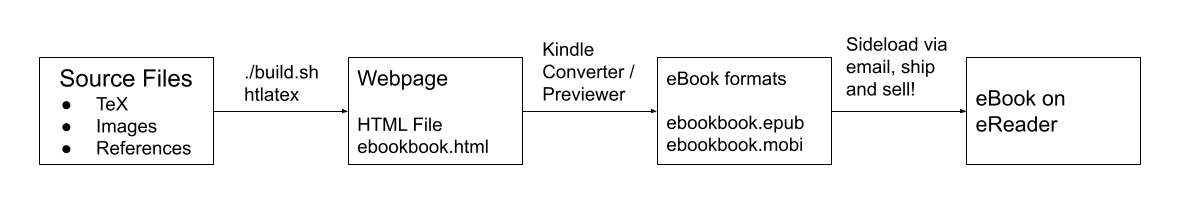
\includegraphics[width=\linewidth]{images/pipeline.png}
\caption{Steps in the pipeline for shipping this ebook}
\label{fig:pipeline}
\end{figure}

The basic outline of the process is shown in Figure \ref{fig:pipeline}.
The rest of this chapter serves to describe the steps in more detail.

The descriptions of commands here will be relatively high-level ---
we'll say things ``install git and run git clone'', rather than giving
details on how to do this on various operating systems. This is for
three reasons. The first is that it's easier to write instructions
this way. The second is that very specific instructions of which web
addresses to visit and which buttons to click on can go stale very
quickly. The third is that this book does assume that the reader has
some experience with and / or tolerance for figuring out a certain
amount of installation and troubleshooting on computers. If not, there are
more constrained off-the-shelf tool that will be easier to get started with
than \latex.

%%
\section{Access and Build the \latex Source}

First of all, you'll want to get a copy of the source code for this
book. (We won't split hairs about whether \latex sources count as
`code'. It gives instructions to machines, it's easy to make mistakes
that show up as error messages, and it's reviewed and stored in source
control --- so it's like code in these practical senses.)

If you already have \texttt{git} installed, this will be something
like running \texttt{git clone
  https://github.com/dwiddows/ebookbook.git} at a command prompt, or
downloading the code using some visual client software. 

List the contents of this directory and check that you can see the
files \texttt{ebookbook.tex} and \texttt{build.sh}. The first of these
is the main \tex document that lays out how to combine the other files
into an ebook.  The second is a build script --- on platforms with
bash or a compatible shell installed, you should be able to run just
\texttt{./build.sh} and get most of the book built using one
command. Or at least, to begin with, you should get error messages
telling you if anything is missing and needs to be installed. If you're not
running a compatible shell, the \texttt{build.sh} will at least give a list
of commands you'll need to run some other way.

So the next step is to run \texttt{./build.sh} and ideally it should
typeset a copy of this book.

%%
\section{From HTML to ePub ... or Mobi}

The most important output from the previous step is a file called \texttt{ebookbook.html}.
This is really formatted for display as a webpage in a browser. This is different
from the more common use of \tex to make documents such as academic papers, which are
nowadays normally created as PDF files.



%%
\chapter{Typesetting Topics}
\label{chapter:typesetting}

This chapter will go through some of the \tex features you'll probably want to use at some point.
So far, {\em most} of the things I usually do with \tex can be made to work for eBook outputs,
but there are lots of commands and options that {\em don't} work and you need to know which
variants to use.

\section{References and Citations}

One of the easy things that `just works' most of the time in \latex is references. For example,
the \tex source for this chapter starts with:

\begin{verbatim}
\chapter{Typesetting Topics}
\label{chapter:typesetting}
\end{verbatim}

Then if I want to refer to the chapter, I write \smalltt{Chapter \textbackslash ref\{chapter:typesetting\}} which
gets rendered as `Chapter \ref{chapter:typesetting}'. Adding \smalltt{label} commands for tables and figures
works in the same way.

This isn't rocket science, but if you've ever tried
renumbering by-hand, you know how valuable this is! Similarly, bibliographic references such as
\smalltt{\textbackslash cite\{knuth1984texbook\}} work correctly, giving a citation looking like \cite{knuth1984texbook}.
I dare say there are plenty of corner cases with bibliography packages, but so far \textsc{BibTeX} has worked
fine for this book.

%%
\section{Graphics}

Nearly all eBooks have graphics in them somewhere, even if just for a cover page. 
The \smalltt{graphicx} works well for this, so for example, the cover image for the title page
of this book is included using the command:

\begin{verbatim}

\includegraphics[width=0.8\linewidth]{images/cover.png}
\end{verbatim}

Typically for webpages and eBooks, the size of images is expected to vary with the page size and settings,
so using a context-sensitive width like a proportion of the linewidth is more appropriate than a fixed-width
declaration like `10cm'. Many eReaders enable users to click on images to see them in more detail, which helps.

One frequent problem is that HTML typesetting using \smalltt{htlatex} or a similar process doesn't always preserve the
aspect ratio of your images. For example, the same setting may be used for width and height, making all images square.
The problem is solved by adding a bounding box file using the \smalltt{extractbb} command, which is typically included
with \tex distributions. This step is included in the project's \smalltt{build.sh} script, at least for \smalltt{.jpg} and
\smalltt{.png} files, and it can easily be extended to more filetypes. Or you can run \smalltt{extractbb -x \$IMAGE} on these files
yourself.

Images are often put in the \latex \smalltt{figure} environment, which can include captions and a label for references.
For example, the map in Figure \ref{fig:sea_map} is created using the commands:

\begin{verbatim}
\begin{figure}
\begin{center}
\caption{A map showing countries in Southeast Asia, 
         made using the \smalltt{pilmaps} library}
  \label{fig:sea_map}
  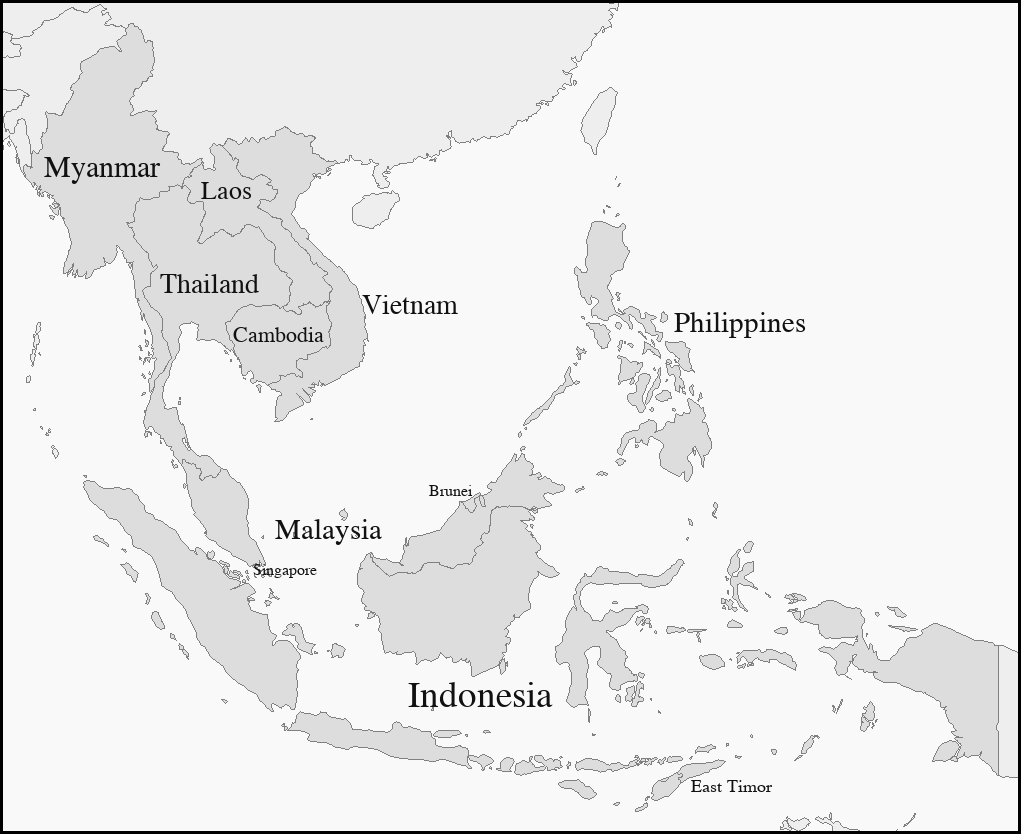
\includegraphics[width=\linewidth]{images/sea_countries.png}
\end{center}
\end{figure}
\end{verbatim}
  
\begin{figure}
\begin{center}
\caption{A map showing countries in Southeast Asia, 
         made using the \smalltt{pilmaps} library}
  \label{fig:sea_map}
  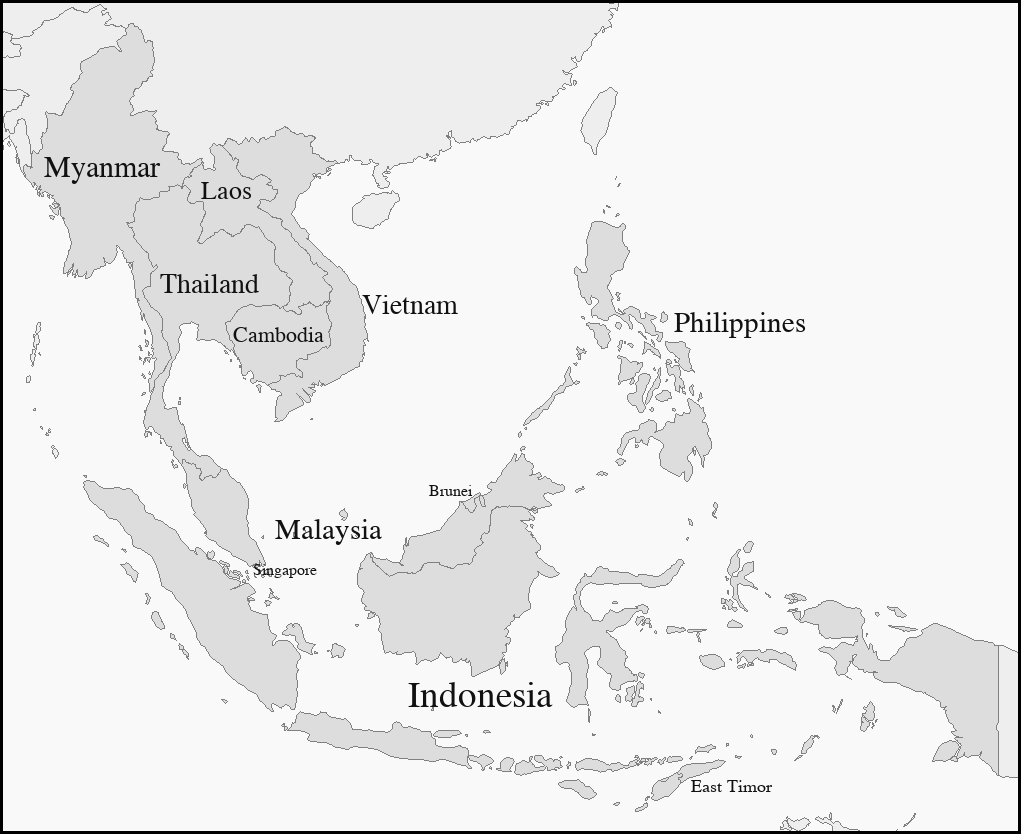
\includegraphics[width=\linewidth]{images/sea_countries.png}
\end{center}
\end{figure}

From here, the figure can be referenced using the command 
\smalltt{\textbackslash ref\{fig:sea\_map\}}. (And if you happen to be looking for a free mapping tool in python that
with low-level, hands-on rendering control, feel free to try {\small \url{https://github.com/dwiddows/pilmaps}}.) 
So far I haven't found an effective way of controlling the placement of figures --- for example, directives
like \smalltt{\textbackslash begin[ht]\{figure\}} don't affect the HTML or the ePub output.

 %%
\section{Tables}

Basic tables typeset just fine. For example, the following \latex gives the output in Table \ref{tab:artist_works}.

\begin{verbatim}
\begin{table}
  \centering
  \begin{tabular}{|c|l|}
    \hline
    \textbf{Artist} & \textbf{Great Works} \\
    \hline
    Leonardo da Vinci & The Mona Lisa \\
    Charlie Watts & Satisfaction \\
    \hline
  \end{tabular}
  \caption{Contributions to modern civilization}
  \label{tab:artist_works}
\end{table}
\end{verbatim}

\begin{table}
 \begin{center}
  \begin{tabular}{|c|l|}
    \hline
    \textbf{Artist} & \textbf{Great Works} \\
    \hline
    Leonardo da Vinci & The Mona Lisa \\
    Charlie Watts & Satisfaction \\
    \hline
  \end{tabular}
  \caption{Contributions to modern civilization}
  \label{tab:artist_works}
 \end{center}
\end{table}

With standard \latex it is easy to make tables that are too big for pages and typeset poorly for a variety of reasons.
I expect this can be even more of a problem with small-screen eBooks, so you'll want to design any tables accordingly
and check output carefully.

%%
\section{Equations}

One of the great draws of \latex is that it's easy to typeset mathematical notation like formulae and equations.

So far these look to work well in HTML and eBook formats. The commands below give the subsequent
renderings of Euler's formula and Fourier series:

\begin{verbatim}
\[ e^{ix} = \cos x + i \sin x \]
\[ f(x) = \sum_{0}^{\infty}a_k \sin(kx) + b_k \cos(kx). \]
\end{verbatim}

\[ e^{i\pi} = -1 \]
\[ f(x) = \sum_{0}^{\infty}a_k \sin(kx) + b_k \cos(kx). \]

Array environments for typesetting rows and columns in equations also work, for example:

\[
u = \left( \begin{array}{c} 1 \\ 0 \\ -2 \end{array} \right) \qquad
v = \left( \begin{array}{c} 2 \\ -1 \\ 3 \end{array} \right) \qquad
u^T v = 2 + 0 - 6 = -4 \qquad
u v^T = \left( \begin{array}{ccc} 2 & -1 & 3 \\ 0 & 0 & 0 \\ -4 & 2 & -6 \end{array} \right)
\]

This set of equations may become typeset in a smaller font than those above, to fit them
horizontally on a small screen. If these start to get too small, consider breaking lines up
when typesetting mathematics for eBooks.

%%
\section{Contents and Index}

The table of contents should get typeset entirely automatically if you use this template.

The story of how traditional indexes and concordances influenced the design of the inverted
indexes used by search engines is quite fascinating, as told by \citet[Ch 1]{witten1999gigabytes}.
Since this story is so advanced by now, I'm not even bothering with an explicit index section ---
if the reader wants to looks something up, use the Search button! If you want to make a paper
version of your book as well, however, you may want to reconsider this.

If you do want to make a paper book as well, it may be worth trying a
more sophisticated template such as the one that comes with Clemens
Lode's book on using \latex for books and eBooks \citep{lode2019better}.

%%%
\chapter{Using \latex for eBooks: Some Things to Avoid}

TODO: Complete and clean up at the end.

Not everything works. If you've used computers for a while, this is not a surprise. In particular in this case,
not everything that works in \latex for (say) PDF documents works for HTML and eBooks.

Things noticed in writing this book that should be avoided or figured out:

\begin{itemize}
    \item The traditional \latex command itself doesn't work.
    \item Footnotes are hard to get on the same page, even with -fn-in option.
    \item Getting a thumbnail image to compile automatically into the e-book format hasn't worked for me.
      TODO: See if this has to be done manually for each publisher.
    \item Boxes produced with the \texttt{wrapfig} package took up the whole width of the page, so marginal boxes didn't work properly this way. 
\end{itemize}





\nextpage
\backmatter

\bibliographystyle{apalike}
\bibliography{bibliography.bib}

\end{document}
